% Created by tikzDevice version 0.12.3.1 on 2021-04-09 22:35:36
% !TEX encoding = UTF-8 Unicode
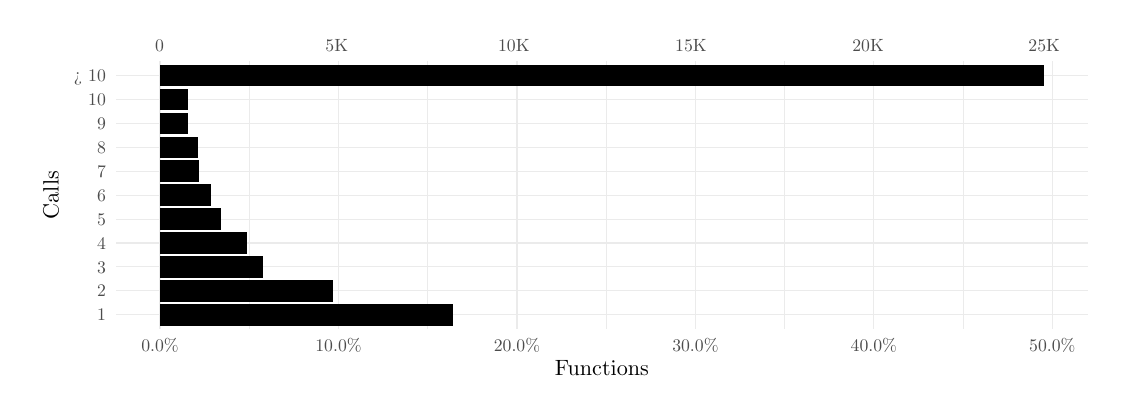
\begin{tikzpicture}[x=1pt,y=1pt]
\definecolor{fillColor}{RGB}{255,255,255}
\path[use as bounding box,fill=fillColor,fill opacity=0.00] (0,0) rectangle (390.26,130.09);
\begin{scope}
\path[clip] ( 31.86, 21.16) rectangle (383.14,117.99);
\definecolor{drawColor}{gray}{0.92}

\path[draw=drawColor,line width= 0.2pt,line join=round] ( 80.07, 21.16) --
	( 80.07,117.99);

\path[draw=drawColor,line width= 0.2pt,line join=round] (144.56, 21.16) --
	(144.56,117.99);

\path[draw=drawColor,line width= 0.2pt,line join=round] (209.04, 21.16) --
	(209.04,117.99);

\path[draw=drawColor,line width= 0.2pt,line join=round] (273.53, 21.16) --
	(273.53,117.99);

\path[draw=drawColor,line width= 0.2pt,line join=round] (338.01, 21.16) --
	(338.01,117.99);

\path[draw=drawColor,line width= 0.4pt,line join=round] ( 31.86, 26.35) --
	(383.14, 26.35);

\path[draw=drawColor,line width= 0.4pt,line join=round] ( 31.86, 34.99) --
	(383.14, 34.99);

\path[draw=drawColor,line width= 0.4pt,line join=round] ( 31.86, 43.64) --
	(383.14, 43.64);

\path[draw=drawColor,line width= 0.4pt,line join=round] ( 31.86, 52.29) --
	(383.14, 52.29);

\path[draw=drawColor,line width= 0.4pt,line join=round] ( 31.86, 60.93) --
	(383.14, 60.93);

\path[draw=drawColor,line width= 0.4pt,line join=round] ( 31.86, 69.58) --
	(383.14, 69.58);

\path[draw=drawColor,line width= 0.4pt,line join=round] ( 31.86, 78.22) --
	(383.14, 78.22);

\path[draw=drawColor,line width= 0.4pt,line join=round] ( 31.86, 86.87) --
	(383.14, 86.87);

\path[draw=drawColor,line width= 0.4pt,line join=round] ( 31.86, 95.51) --
	(383.14, 95.51);

\path[draw=drawColor,line width= 0.4pt,line join=round] ( 31.86,104.16) --
	(383.14,104.16);

\path[draw=drawColor,line width= 0.4pt,line join=round] ( 31.86,112.80) --
	(383.14,112.80);

\path[draw=drawColor,line width= 0.4pt,line join=round] ( 47.83, 21.16) --
	( 47.83,117.99);

\path[draw=drawColor,line width= 0.4pt,line join=round] (112.32, 21.16) --
	(112.32,117.99);

\path[draw=drawColor,line width= 0.4pt,line join=round] (176.80, 21.16) --
	(176.80,117.99);

\path[draw=drawColor,line width= 0.4pt,line join=round] (241.28, 21.16) --
	(241.28,117.99);

\path[draw=drawColor,line width= 0.4pt,line join=round] (305.77, 21.16) --
	(305.77,117.99);

\path[draw=drawColor,line width= 0.4pt,line join=round] (370.25, 21.16) --
	(370.25,117.99);
\definecolor{fillColor}{RGB}{0,0,0}

\path[fill=fillColor] ( 47.83,108.91) rectangle (367.18,116.69);

\path[fill=fillColor] ( 47.83, 22.46) rectangle (153.54, 30.24);

\path[fill=fillColor] ( 47.83,100.27) rectangle ( 58.11,108.05);

\path[fill=fillColor] ( 47.83, 31.10) rectangle (110.49, 38.88);

\path[fill=fillColor] ( 47.83, 39.75) rectangle ( 84.95, 47.53);

\path[fill=fillColor] ( 47.83, 48.39) rectangle ( 79.17, 56.18);

\path[fill=fillColor] ( 47.83, 57.04) rectangle ( 69.98, 64.82);

\path[fill=fillColor] ( 47.83, 65.69) rectangle ( 66.25, 73.47);

\path[fill=fillColor] ( 47.83, 74.33) rectangle ( 62.02, 82.11);

\path[fill=fillColor] ( 47.83, 82.98) rectangle ( 61.49, 90.76);

\path[fill=fillColor] ( 47.83, 91.62) rectangle ( 57.80, 99.40);
\end{scope}
\begin{scope}
\path[clip] (  0.00,  0.00) rectangle (390.26,130.09);
\definecolor{drawColor}{gray}{0.30}

\node[text=drawColor,anchor=base,inner sep=0pt, outer sep=0pt, scale=  0.64] at ( 47.69,121.59) {0};

\node[text=drawColor,anchor=base,inner sep=0pt, outer sep=0pt, scale=  0.64] at (111.68,121.59) {5K};

\node[text=drawColor,anchor=base,inner sep=0pt, outer sep=0pt, scale=  0.64] at (175.68,121.59) {10K};

\node[text=drawColor,anchor=base,inner sep=0pt, outer sep=0pt, scale=  0.64] at (239.68,121.59) {15K};

\node[text=drawColor,anchor=base,inner sep=0pt, outer sep=0pt, scale=  0.64] at (303.68,121.59) {20K};

\node[text=drawColor,anchor=base,inner sep=0pt, outer sep=0pt, scale=  0.64] at (367.32,121.59) {25K};
\end{scope}
\begin{scope}
\path[clip] (  0.00,  0.00) rectangle (390.26,130.09);
\definecolor{drawColor}{gray}{0.30}

\node[text=drawColor,anchor=base east,inner sep=0pt, outer sep=0pt, scale=  0.64] at ( 28.26, 24.15) {1};

\node[text=drawColor,anchor=base east,inner sep=0pt, outer sep=0pt, scale=  0.64] at ( 28.26, 32.79) {2};

\node[text=drawColor,anchor=base east,inner sep=0pt, outer sep=0pt, scale=  0.64] at ( 28.26, 41.44) {3};

\node[text=drawColor,anchor=base east,inner sep=0pt, outer sep=0pt, scale=  0.64] at ( 28.26, 50.08) {4};

\node[text=drawColor,anchor=base east,inner sep=0pt, outer sep=0pt, scale=  0.64] at ( 28.26, 58.73) {5};

\node[text=drawColor,anchor=base east,inner sep=0pt, outer sep=0pt, scale=  0.64] at ( 28.26, 67.37) {6};

\node[text=drawColor,anchor=base east,inner sep=0pt, outer sep=0pt, scale=  0.64] at ( 28.26, 76.02) {7};

\node[text=drawColor,anchor=base east,inner sep=0pt, outer sep=0pt, scale=  0.64] at ( 28.26, 84.66) {8};

\node[text=drawColor,anchor=base east,inner sep=0pt, outer sep=0pt, scale=  0.64] at ( 28.26, 93.31) {9};

\node[text=drawColor,anchor=base east,inner sep=0pt, outer sep=0pt, scale=  0.64] at ( 28.26,101.95) {10};

\node[text=drawColor,anchor=base east,inner sep=0pt, outer sep=0pt, scale=  0.64] at ( 28.26,110.60) {> 10};
\end{scope}
\begin{scope}
\path[clip] (  0.00,  0.00) rectangle (390.26,130.09);
\definecolor{drawColor}{gray}{0.30}

\node[text=drawColor,anchor=base,inner sep=0pt, outer sep=0pt, scale=  0.64] at ( 47.83, 13.15) {0.0{\%}};

\node[text=drawColor,anchor=base,inner sep=0pt, outer sep=0pt, scale=  0.64] at (112.32, 13.15) {10.0{\%}};

\node[text=drawColor,anchor=base,inner sep=0pt, outer sep=0pt, scale=  0.64] at (176.80, 13.15) {20.0{\%}};

\node[text=drawColor,anchor=base,inner sep=0pt, outer sep=0pt, scale=  0.64] at (241.28, 13.15) {30.0{\%}};

\node[text=drawColor,anchor=base,inner sep=0pt, outer sep=0pt, scale=  0.64] at (305.77, 13.15) {40.0{\%}};

\node[text=drawColor,anchor=base,inner sep=0pt, outer sep=0pt, scale=  0.64] at (370.25, 13.15) {50.0{\%}};
\end{scope}
\begin{scope}
\path[clip] (  0.00,  0.00) rectangle (390.26,130.09);
\definecolor{drawColor}{RGB}{0,0,0}

\node[text=drawColor,anchor=base,inner sep=0pt, outer sep=0pt, scale=  0.80] at (207.50,  4.40) {Functions};
\end{scope}
\begin{scope}
\path[clip] (  0.00,  0.00) rectangle (390.26,130.09);
\definecolor{drawColor}{RGB}{0,0,0}

\node[text=drawColor,rotate= 90.00,anchor=base,inner sep=0pt, outer sep=0pt, scale=  0.80] at ( 11.20, 69.58) {Calls};
\end{scope}
\end{tikzpicture}
